\chapter{Part II: Storage Format Enhancement}
\label{chap:storage-format}
In the previous chapter, we concluded that there was potential in column storage in \gap, but that more memory could be saved by enhancing the data storage format. In this chapter, we show how memory usage is reduced and memory locality improved by replacing \cn{GValue}s with primitive data types. We also study the effect of loading raw string values from XML directly into the columns.

This chapter forms the second iteration of our design and experiment part of the research. In this iteration, we are mainly pursuing reduced memory footprint, but the modifications from the storage format enhancements serve as an important foundation for column operations, which we discuss in Chapter \ref{chap:operations}.  
\clearpage

\section{Introduction}
\label{sec:Introduction}
In Section \ref{sec:Challenges in Genus App Platform}, we saw that two of the challenges in the original \gap~data representation are poor memory locality and inefficient storage usage. Both challenges are caused by the \cn{GValue} class. In this structure, data is stored inefficiently due to overhead of pointers and reference counting. For example, it takes 24 bytes to store a 4 byte integer. Secondly, since \cn{GValue} is a class type, it is heap allocated by the memory manager, and we have no control over where the values reside in memory. In Chapter \ref{chap:olap}, we saw that spatial and temporal locality is paramount for performance.

One might think that memory locality and cache hit rate have been improved by the introduction of \cn{FieldValueCollection} in the previous chapter. This is only partially true; we store value pointers consecutively in memory with the \cn{TArray} type, but the structures containing the data itself reside in arbitrary memory locations.

Section \ref{sub:Delphi Types} explained that \delphi~supports a wide range of simple, or primitive, data types. These include integer, character, Boolean, real, and more. Common for these data types is that they are value types and a variable with one such type stores the data directly, and not as a pointer to the heap. This is also the case for the \delphi~\cn{record} type.

We observe that if we change the value buffers in \cn{FieldValueCollection} from holding \cn{GValue} references to storing primitive value types directly, we overcome the above challenges. First, we reduce memory consumption by transitioning to primitive data types, since these values have no pointer or reference counting overhead. Second, since we plan to store the values directly in \delphi~array structures, we improve memory locality.

The data source loading mechanism in \gap~operates with \cn{GValue}s, but since we plan to no longer use this class to represent data in a data source, we are curious to see whether \cn{GValue}s can be eliminated from the data load process. We believe data load time can be reduced by loading the database values directly from XML instead of using \cn{GValue}s to load values into columns.

Motivated by the memory reduction and the ability to regain control over memory, we create a new structure based on the \cn{FieldValueCollection} interface, which we denote as \cn{PrimitiveFieldValueCollection}. We also circumvent \cn{GValue} creation in the \gap~load module and pass raw XML values directly to the columns. We hypothesize that these changes will reduce memory consumption and decrease load time.

\section{Implementation}
\label{sec:Implementation}
In this section, we start by explaining the \cn{PrimitiveFieldValueCollection} column class and how \gap~selects the correct primitive column type. Then we elaborate on how we circumvent \cn{GValue} creation in the data load module.

\subsection{PrimitiveFieldValueCollection}
\label{sub:PrimitiveFieldValueCollection}

\afigure{img/primitive-hierarchy.png}{Column store class hierarchy after the introduction of primitive data type support. \cn{FieldValueCollection} and \cn{PrimitiveFieldValueCollection} extends a common base class, \cn{FieldValueCollectionBase}. \cn{PrimitiveFieldValueCollection} has one subclass per supported primitive data type. Although string is not a simple data type in \delphi, we still create a string primitive column subclass. The primitive value column structure still has an \cn{GValue} interface in getters and setters.}{fig:primitive-hierarchy}{1.0}

To add primitive data type support to our column store, we extract core column functionality to an abstract class \cn{FieldValueCollectionBase}. Then, we introduce a new class that extends from this base class, \cn{PrimitiveFieldValueCollection}. This class is a generic class with a subclass for every supported data type. The hierarchy is shown in Figure \ref{fig:primitive-hierarchy}.

\begin{delphicode}{\fn{GetValue} function in \cn{PrimitiveFieldValueCollection}.}{lst:primitive-get-value}
function PrimitiveFieldValueCollectionBase<TType>.GetValue
( index : integer )
: CGValue;
begin
  EnsureCapacity(index);
  if not nilFlags[index] then
    Result := valueHelper.CreateCGValue(values[index])
  else
    Result := nil;
end;
\end{delphicode}

\cn{PrimitiveFieldValueCollection} holds all data in a \cn{TArray} of the primitive data type of choice. However, \fn{GetValue} and \fn{SetValue} methods still use \cn{GValue} as return and input types respectively. To help isolate all code related to value conversion and avoid code duplication, we create a value helper class which we instantiate in all primitive column subclasses. This class contains methods for extracting primitive data values from a \cn{GValue}, creating \cn{GValue}s based using primitive data types as input, as well as some simple comparison operators. We have provided an example of how it is used in Listing \ref{lst:primitive-get-value}. Like \cn{PrimitiveFieldValueCollection}, the class is generic, with subclasses for every supported data type.

In the last iteration, we introduced the \vn{nilFlags} bitmap. Whereas \cn{FieldValueCollection} could store \null~pointers in the value buffers instead of pointers to \cn{GValue}s, we no longer have this opportunity, as simple value types in \delphi~are not nullable. Hence, \vn{nilFlags} bitmap is used to indicate which values are null. As seen in Listing \ref{lst:primitive-get-value}, the flags are checked before creating a value.

Even though they are not considered as simple data types in \delphi, we apply the same techniques for strings and records. Record types, like \vn{TGuid}, have value semantics and work similarly as simple data types, which means they are allocated consecutively in memory using the \cn{TArray} type. Strings, however, are pointer types, which means pointers are stored consecutively in the columns, but not the data itself. Hence, we do not get the benefit from explicit memory control on strings, but we remove an extra layer of indirection to access a value and avoid the overhead related to \cn{GValue}.

\subsection{Column Selection}
\label{sub:Column Selection}
To make the new \cn{PrimitiveFieldValueCollection} class work, we must pick the correct primitive type subclass for the different data descriptors in a data source. This is the responsibility of the column store. We extend \cn{CompositionValueCollection} with a \fn{GetFieldValueCollection} which takes a data descriptor as an input and returns the correct column. In this method, the data descriptor is queried for its data type, and it picks the correct \cn{PrimitiveFieldValueCollection} subclass. If no matching primitive data type column is found, the method falls back on the original \cn{FieldValueCollection} from Chapter \ref{chap:column-store}.

\subsection{Loading Raw XML Values Directly}
\label{storage-format:raw-xml}
\begin{figure}
    \centering
    \begin{subfigure}{\textwidth}
        \centering
        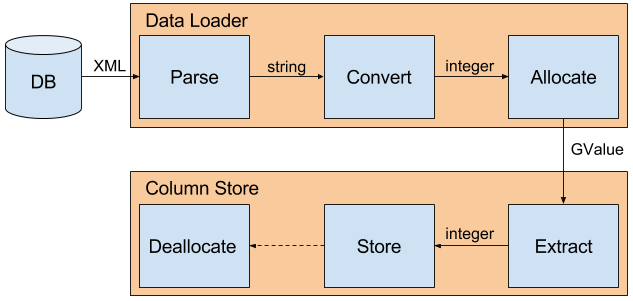
\includegraphics[width=0.8\textwidth]{img/gap-load-original.png}
        \caption{Original implementation where all data is transferred as \cn{GValue}s.}
    \end{subfigure}
    \begin{subfigure}{\textwidth}
        \centering
        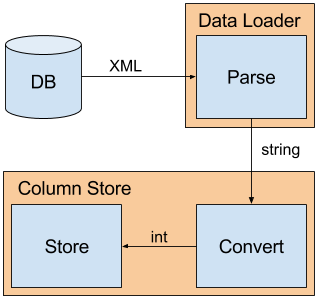
\includegraphics[width=0.4\textwidth]{img/gap-load-raw.png}
        \caption{Enhanced implementation where data is passed to the column store as strings.}
    \end{subfigure}
\caption{By loading raw XML strings directly into the columns, the load process is simplified, and we remove uneccessary memory allocations for \cn{GValue}.}
\label{fig:gap-load-raw}
\end{figure}

In \gap, composition objects in a data source are populated with data using a loading mechanism found in the platform's event handler. We refer to this mechanism as the \textit{data loader}. The data loader queries the database infrastructure for data which is returned as XML. The loader parses the XML into strings, converts the values to the correct value type, and allocates \cn{GValue}s, as seen in Figure \ref{fig:gap-load-raw}a. Our observation is, with the primitive data type column implementation, that \cn{GValue}s are surplus and causes additional memory management overhead.

\begin{delphicode}{\fn{SetXMLValue} in \cn{PrimitiveFieldValueCollection}.}{lst:primitive-set-xml-value}
procedure PrimitiveFieldValueCollection<TType>.SetXMLValue
( index : integer; xmlValue : string);
begin
  EnsureCapacity(index);
  values[index] := valueHelper.GetFromXMLValue(xmlValue);
  nilFlags[index] := FALSE;
  assignedFlags[index] := TRUE;
end;
\end{delphicode}
Hence, we extend the \cn{FieldValueCollectionBase} interface with a new method, \fn{LoadXMLValue}, which accepts a data source index as well as a string XML value as inputs. The value helper class is also extended accordingly. For the different primitive data types, this method is overridden and implemented with high performance standard library functions, like \fn{StrToInt} and \fn{StrToFloat}. For more advanced data types, like date, the correct \gap~parser functions are used. We see the \fn{SetXMLValue} implementation in Listing \ref{lst:primitive-set-xml-value}.

As a result of our changes, the loading process has been simplified and memory allocations reduced. See Figure \ref{fig:gap-load-raw}.
\section{Results}
\label{sec:storage-format-test-results}
Like the previous iteration, we assess our modifications by using Benchmark \ref{bm:q1}, the \tpchdl. We use this benchmark to test our hypothesis that primitive value storage and direct value load contribute to reduced memory footprint and improved load time. 

\cn{GetValue} and \cn{SetValue} in \cn{PrimitiveFieldValueCollection} still use a \cn{GValue} interface, which means memory for the \cn{GValue} is allocated and deallocated on each method call respectively. We are, therefore, interested in testing the effects of this extra memory handling operations with Benchmark \ref{bm:write}, the \textit{Write Benchmark}. We also believe the read-intense operations, join and source measure lookup, in Benchmark \ref{bm:q1} provides insight on this matter.

We test two configurations in this iteration which is the new primitive value column implementation with and without raw XML value load. We denote the configurations as \textit{primitive w/ raw load} and \textit{primitive} respectively. We compare the benchmark results with the previous iteration, and we denote the configuration from this iteration as \textit{column store}. Due to time constraints, we run the benchmarks only three times and report the average result. However, all measurements had low variance with no outliers.

Full benchmark details are found in Appendix \ref{app:bm}.

\subsection{Data Mart Load Benchmark}
\label{storage-format:q1}

Benchmark \ref{bm:q1} was run with the new primitive value column implementation, with and without the new loading scheme. We run both scaling factors SF0.01 and SF0.1, but if we observe the same effects on both scaling factors, we only report for SF0.1.

\afigure{img/storage-format-bpl.png}{Bytes per \lineitem~used by the \cn{FieldValueCollection} implementation from Chapter \ref{chap:column-store}, primitive value columns, and primitive value columns with raw XML data load, Benchmark \ref{bm:q1} with scaling factors SF0.01 and SF0.1.}{fig:storage-format-bpl}{0.9}
As seen in Figure \ref{fig:storage-format-bpl}, primitive value columns reduce memory consumption per \lineitem~from 419 to 333 bytes and from 501 to 374 bytes for scaling factors SF0.01 and SF0.1 respectively. This corresponds to 21 \% and 25 \% reduction in memory footprint. However, the \textit{primitive w/ raw load} configuration does not reduce the bytes per \lineitem~as much as the \textit{primitive} configuration, although it is still lower than the original column store.

\afigure{img/storage-format-load.png}{Data source load time for the \cn{FieldValueCollection} from Chapter \ref{chap:column-store}, primitive value columns, and primitive value columns with raw XML data load, Benchmark \ref{bm:q1}, SF0.1.}{fig:storage-format-load}{0.7}

Load times are increased by the primitive column store, but it is still lower than the original \gap~row storage implementation. However, with our raw XML loading mechanisms, the load time has increased even more, and is comparable original implementation. The results are presented in Figure \ref{fig:storage-format-load}. 

\afigure{img/storage-format-lig.png}{Lookup index generation performance for the \cn{FieldValueCollection} from Chapter \ref{chap:column-store} and primitive value columns, Benchmark \ref{bm:q1}, SF0.1.}{fig:storage-format-lig}{0.9}
\afigure{img/storage-format-sml.png}{Source measure lookup performance for the \cn{FieldValueCollection} from Chapter \ref{chap:column-store} and primitive value columns, Benchmark \ref{bm:q1}, SF0.1.}{fig:storage-format-sml}{1.0}

Both read-intense operations in \tpchdl~are drastically slowed down by the new primitive value storage format. As seen in Figure \ref{fig:storage-format-lig}, lookup index generation performs 3-4 times worse than the \cn{FieldValueCollection} implementation. Sorce measure lookup sees an even higher performance impact, and is, according to Figure \ref{fig:storage-format-sml}, ten times slower as the implementation of the previous chapter, and almost 20 times slower as the original \gap.

\subsection{Write Benchmark}
\label{sub:Write Benchmark}
\afigure{img/storage-format-write.png}{Write performance for the \cn{FieldValueCollection} from Chapter \ref{chap:column-store} and primitive value columns, Benchmark \ref{bm:write}, 1000 elements.}{fig:storage-format-write}{1.0}
Write performance has, as Figure \ref{fig:storage-format-write} shows, degraded slightly with the new primitive data type column store. However, no operations are more than 15 \% slower than the original.

\section{Discussion}
\label{sec:part2-discussion}

We see that the memory used per \lineitem~for scaling factor SF0.1 has been reduced by an additional 25 \% compared to the \cn{FieldValueCollection} implementation. This observation confirms our hypothesis that the overhead associated with \cn{GValue}s is significant.

We observe an increased load time for Benchmark \ref{bm:q1}, where the time it takes to populate the data source is increased from 8.5 seconds to 13.6 seconds. We believe the extra steps needed to extract raw values from \cn{GValue} instances causes this. Still, the load time is lower than the original \gap~implementation.

Circumventing \cn{GValue} creation and loading raw XML string values directly into the column store had no positive effect on the \tpchdl. Here, both the number of bytes per \lineitem~and load time increased. We did circumvent the creation of \cn{GValue}s, but by doing so, we also disabled the existing caching mechanism in \gap. Thus, no strings are reused, and no conversion results are cached. We find it likely that this is the cause of increased memory usage and load time.

We see the consequences of having a \cn{GValue} interface on the columns, which results in frequent allocations and deallocations when accessing values. The \textit{write benchmark} shows slightly reduced write performance. However, we measure the largest performance impact on the read-intensive operations in the \tpchdl. For source measure lookup, which creates a real value array for a column using a tight loop, the performance has dropped and is now ten times slower than the \cn{FieldValueCollection} column store due to the frequent memory allocations.

%The extra steps of \cn{GValue} allocation and deallocation also affects write performance in Benchmark \ref{bm:write}, although not by more than 15 \%. This indicates that there are much more overhead associated with data write than just allocating \cn{GValue}s.

\section{Iteration Conclusion}
\label{sec:Iteration Conclusion}
We conclude that primitive value column storage successfully reduces memory consumption in \gap. Compared to the original implementation, the bytes used per \lineitem~are reduced from 715 bytes to 374 bytes. Our changes have affected write performance negatively, but not by more than 15 \%. We argue that the significant reduction in memory usage outweighs the slightly negative impact on write performance, and concludes that storing values as primitive data types and using a \cn{GValue} interface is feasible. 

In this iteration, we have laid an important foundation for optimizing the read-intensive operations in the \tpchdl by increasing data locality. More specifically, we have replaced the \cn{GValue} pointers and now store values directly in the columns. Until we exploit this storage structure, source measure lookup and lookup index generation suffer severely due to memory allocation operations on each access. We investigate column operations in Chapter \ref{chap:operations}.

Our hypothesis that loading data as raw XML values into the column would reduce load time was wrong, at least for now. Circumventing \cn{GValue}s also circumvents the built-in caching mechanism in \gap~and results in higher memory usage and slower load times.  

We have cut the application memory requirements in half without applying any form of compression. Now that we know data can be stored as primitive data types, the next step is to compress the data with techniques used by read-optimized databases.

\subsection{Future Work}
\label{sub:Future Work}
We are still keen to investigate the potential of loading XML values directly, but due to time constraints, we are unable to pursue this topic further. Future work should aim to replicate the existing caching mechanisms in \gap, but within the column store and without creation of \cn{GValue}s. Caching could, for instance, only be enabled if the data source is in a feeding state. Building on the idea of horizontal partitioning from Section \ref{sub:column-store:future-work}, caching could also be used in newly created partitions, and once a partition is full, all caching structures are discarded and the partition is optimized for read-only workloads.

%\begin{table}
%    \begin{tabularx}{\textwidth}{X | X X X X}
%         & \texttt{QUANTITY} & \texttt{EXTENDEDPRICE} & \texttt{COMMENT} & \texttt{SHIPDATE}\\ 
%        \hline
%        \hline
%        Column Store & 1642 ms & 1610 ms & 1770 ms & 2046 ms \\
%        Primitive Column Store & 1807 ms & 1779 ms & 1820 ms & 2352 ms \\
%    \end{tabularx}
%    \caption{Test results for Benchmark \ref{bm:write}.}
%    \label{tab:primitive-write}
%\end{table}
%Most operations are drastically slowed down by the new primitive storage format, as seen in Table \ref{tab:primitive-q1}. Source measure lookup is ten times slower than the previous column store implementation, and almost 20 times slower as the original implementation.
%We are surprised to see that our new loading mechanism has degraded load performance. We discuss this in greater detail in Section \ref{sec:part2-discussion}. 
%Benchmark \ref{bm:q1}, the \textit{TPC-H Q1 Data Load Benchmark}, was run with our new primitive value column implementation with and without the new loading scheme. Both scaling factor 0.1 and 0.01 were run. Like in Chapter \ref{chap:column-store}, only three tests were run per configuration. However, all results yielded low variance, and no single measurement was more than 15 \% different than the average value.
%We run Benchmark \ref{bm:q1} with the new primitive value column implementation, and with and without the new loading scheme. We also provide comparisons with the \cn{FieldValueCollection} from the previous chapter.


%\begin{table}
%    \centering
%    \begin{tabularx}{\textwidth}{X | X X}
%        & SF0.01 & SF0.1 \\ 
%        \hline
%        \hline
%        Column Store & 419 bytes & 501 bytes \\
%        Primitive Column Store & 333 bytes & 374 bytes \\
%        Primitive Column Store /w raw load & 381 bytes & 422 bytes \\
%    \end{tabularx}
%    \caption{Bytes per \texttt{LINEITEM} used by the new primitive value implementation.} 
%    \label{tab:primitive-bpl}
%\end{table}

%\begin{table}
%    \centering
%    \begin{tabularx}{0.75\textwidth}{X | X X}
%        & SF0.01 & SF0.1 \\ 
%        \hline
%        \hline
%        Column Store & 842 ms & 8539 ms \\
%        Primitive Column Store & 1210 ms & 13585 ms \\
%        Primitive Column Store w/ raw load &  20966 ms & 2306 ms \\
%    \end{tabularx}
%    \caption{Load times for Benchmark \ref{bm:q1} for the primitive column store for scaling factors 0.01 and 0.1.} 
%    \label{tab:primitive-load}
%\end{table}

%\begin{table}
%    \centering
%    \begin{tabularx}{\textwidth}{X | X X X | X X X X}
%        & \multicolumn{3}{c}{Lookup Index} & \multicolumn{4}{c}{Source Measure Lookup} \\
%        \hline
%        \hline
%        Column Store & 3123 ms & 3301 ms & 13004 ms & 532 ms & 625 ms & 646 ms & 752 ms \\
%        Primitive Column Store & 11393 ms & 11960 ms & 19365 ms & 6556 ms & 6856 ms & 6840 ms & 6826 ms \\
%    \end{tabularx}
%    \caption{Data mart load operation times for \ref{bm:q1} with the primitive columns.} 
%    \label{tab:primitive-q1}
%\end{table}
